\documentclass[9pt]{beamer}

% apparence
\usetheme{Singapore}
\usecolortheme{orchid}
\setbeamercolor{title}{
	use=structure,fg=white,bg=structure.fg!75!black
}
\useinnertheme[shadow]{rounded}

% numéro des slides
\addtobeamertemplate{navigation symbols}{}{
	\usebeamerfont{footline}
	\usebeamercolor[fg]{footline}
	\hspace{1em}
	\raisebox{2pt}{
		\insertframenumber/\inserttotalframenumber
	}
}

\makeatletter

% afficher/masquer dans miniframes
\let\beamer@writeslidentry@miniframeson=\beamer@writeslidentry
\def\beamer@writeslidentry@miniframesoff{
	\expandafter\beamer@ifempty\expandafter{\beamer@framestartpage}{}
	{\clearpage\beamer@notesactions}
}

\newcommand*{\miniframeson}{
	\let\beamer@writeslidentry=\beamer@writeslidentry@miniframeson
}

\newcommand*{\miniframesoff}{
	\let\beamer@writeslidentry=\beamer@writeslidentry@miniframesoff
}

\makeatother

% packages
\usepackage{setspace}
\usepackage{mathtools}
\usepackage{graphicx, multirow}
\usepackage{algorithm, algpseudocode}
\usepackage[dvipsnames]{xcolor}
\usepackage{tikz}
\usepackage{appendixnumberbeamer}

% puces numérotées
\newcommand{\ballbullet}[1]{%
	\tikz[baseline=(n.base)]{
		\shade[ball color=structure.fg] (0,0) circle (1.1ex);
		\node[text=white, inner sep=0pt, scale=0.8] (n) at (0,0) {#1};
	}%
}

% titre du beamer
\title{
	Autonomous Navigation and Mapping over Physical Fields\\
	by Gaussian Process-based Particle Filtering
}

\author{
	\texorpdfstring{
		{\Large Bastien HUBERT\inst{1,2}}\\[\baselineskip]
		\begin{tabular}{rl}
			Supervisor:&Audrey GIREMUS\inst{2}\\
			Co-supervisor:&Karim DAHIA\inst{1}\\
			Advisor:&Nicolas MERLINGE\inst{1}
		\end{tabular}
	}{
		Bastien HUBERT
	}
}

\institute{
	\inst{1} ONERA, DTIS, IGNC\quad
	\inst{2} Université de Bordeaux, CNRS, IMS
}

\date{8 December 2026}

\titlegraphic{
	\vspace{-0.5\baselineskip}
	
\includegraphics[width=10cm]{../../Images/Logo ONERA IMS.pdf}
}

% début du beamer
\begin{document}

\setlength{\abovedisplayskip}{3pt}
\setlength{\belowdisplayskip}{3pt}

\begin{frame}

\titlepage

\end{frame}

\logo{
	
\includegraphics[width=3.8cm]{../../Images/Logo ONERA IMS.pdf}
}

\section{Introduction}

\begin{frame}{Context: autonomous navigation for UAVs}

\begin{block}{Inertial navigation for unmanned aerial vehicles (UAVs)}
	\begin{itemize}
		\item Integrates measurements from the accelerometers and gyroscopes of an inertial measurement unit
		\item Autonomous and reliable over short durations
		\item But imperfect measurements (biases, scale factors, noises, ...)
		\item Drifts over time: \ballbullet{1}
	\end{itemize}
\end{block}

\begin{block}{Data fusion}
	\begin{itemize}
		\item Using data from other sensors helps reduce \ballbullet{1}
		\item Usual counterpart: GNSS, but may be unavailable, jammed or spoofed: \ballbullet{2}
		\item[$\Rightarrow$] Physical field-aided navigation instead
		\item Measurements from an exteroceptive onboard sensor
		\item Comparison between the measured data and an embedded map
	\end{itemize}
\end{block}

\end{frame}

\begin{frame}{Physical field-aided navigation}

\begin{columns}[onlytextwidth,T]
	\begin{column}{0.48\textwidth}

		\begin{block}{Terrain-aided navigation}
			\begin{itemize}
			\item Sensor: radar altimeter
			\item Measurement: overflown terrain altitude
			\end{itemize}
		\end{block}

	\end{column}
	\begin{column}{0.48\textwidth}

		\begin{block}{Magnetic anomaly-aided navigation}
			\begin{itemize}
				\item Sensor: Magnetometer
				\item Measurement: Earth's magnetic anomaly:
				\hfill\scalebox{0.85}{$\mathcal{B}=\mathcal{B}_{\mathrm{core}}+\boxed{\mathcal{B}_{\mathrm{crust}}}+\mathcal{B}_{\mathrm{vehicle}}+\mathcal{B}_{\mathrm{ext}}$}\hfill\mbox{}
			\end{itemize}
		\end{block}

	\end{column}
\end{columns}

\begin{columns}[onlytextwidth]
	\begin{column}{0.48\textwidth}

		\centering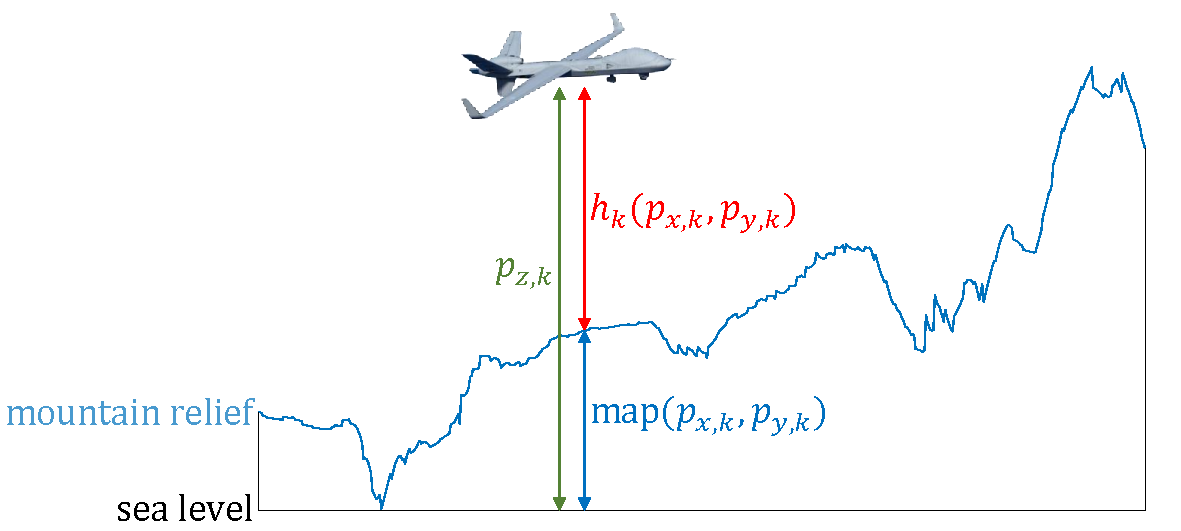
\includegraphics[width=\textwidth]{../../Images/Schéma de la corrélation de terrain.pdf}

	\end{column}
	\begin{column}{0.48\textwidth}

		\centering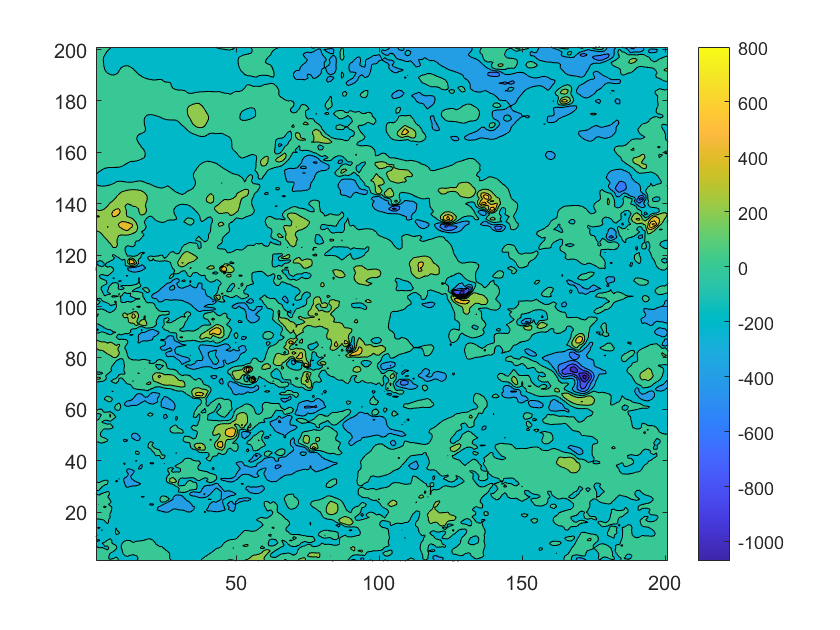
\includegraphics[width=0.7\textwidth]{../../Images/Carte magnétométrique EUSIPCO 2025.png}

	\end{column}
\end{columns}

\begin{block}{Challenges}
	\begin{itemize}
		\item Large initial state uncertainty: \ballbullet{3}
		\item Non-linear and non-injective environment model: \ballbullet{4}
		\item Sparse and noisy knowledge of the field: \ballbullet{5} or no knowledge at all: \ballbullet{6}
	\end{itemize}
\end{block}

\end{frame}

\begin{frame}{Problem statement}

\begin{block}{Discrete state-space model}
	\begin{equation}
		\left\{\begin{aligned}
		x_k&=f_k(x_{k-1},\eta_k)&&\text{recursive evolution process}\\
		z_k&=h_k(x_k,\varepsilon_k)&&\text{observation function}
		\end{aligned}\right.
	\end{equation}
	\begin{itemize}
		\item Goal: recursively estimate the state $x_k$ (position, velocity, ... of the UAV) given the observations $\mathbf{z}_{1:k}=(z_1,\dots,z_k)$
	\end{itemize}
\end{block}

\begin{block}{Knowledge of the environment}
	\begin{itemize}
		\item Known field, standard case: $h_k$ is known and an embedded map is available
		\item Poorly known field (\ballbullet{5}): $h_k$ only known through undersampled noisy data $(\tilde{\mathbf{x}},\tilde{\mathbf{z}})$ and must be reconstructed
		\item Unknown field (\ballbullet{6}): $h_k$ is completely unknown and must be learnt online, concurrently with the state (SLAM)
	\end{itemize}
\end{block}

\end{frame}

\begin{frame}{Objectives and outline}

\begin{block}{Research objectives}
	\begin{itemize}
		\item Explore mathematical representations of physical fields and quantify the approximation errors
		\item Develop robust and tractable navigation solutions for \ballbullet{5}
		\item Extend such methods to \ballbullet{6}
	\end{itemize}
\end{block}

\begin{block}{Outline}
	\begin{itemize}
		\item Background: Bayesian estimation and Gaussian processes
		\item Navigation over a poorly known environment: naive and adaptive methods
		\item Navigation over an unknown environment
		\item Conclusion and perspectives
	\end{itemize}
\end{block}

\end{frame}

\section{Bayesian estimation}

\begin{frame}{Bayesian estimation}

\begin{block}{State estimation}
	\begin{itemize}
		\item Minimum mean squared error (MMSE) of $x_k$ given $\mathbf{z}_{1:k}$:
		\begin{equation}
			\underset{\psi\in\mathcal{L}^2}{\operatorname{argmin}}\left\{\mathbb{E}\left[\|\psi(\mathbf{z}_{1:k})-x_k\|^2\right]\right\}=\mathbb{E}\left[x_k\mid\mathbf{z}_{1:k}\right]=\int x_k\:p(x_k\mid\mathbf{z}_{1:k})\:dx_k
		\end{equation}
		\item Goal: compute the posterior density $p(x_k\mid\mathbf{z}_{1:k})$ to address \ballbullet{3} and \ballbullet{4}
	\end{itemize}
\end{block}

\begin{block}{Optimal Bayesian filter}
	\begin{itemize}
	\item Prediction with the Chapman-Kolmogorov equation:
	\begin{equation}
		p(x_k\mid\mathbf{z}_{1:k-1})=\underbrace{\int p(x_k\mid x_{k-1})\:p(x_{k-1}\mid\mathbf{z}_{1:k-1})\:dx_{k-1}}_{\text{no analytical solution in general}}
	\end{equation}
	\item Correction with Bayes' formula:
	\begin{equation}
		p(x_k\mid\mathbf{z}_{1:k})\propto\underbrace{p(z_k\mid x_k)}_{\text{requires }h_k\text{\rlap{ so cannot be applied to {\ballbullet{5}} or \ballbullet{6}}}}\:p(x_k\mid\mathbf{z}_{1:k-1})
	\end{equation}
	\end{itemize}
\end{block}

\end{frame}

\begin{frame}{Analytical filtering}

\begin{block}{Kalman filter}
	\begin{itemize}
	\item Optimal recursive estimation under linear Gaussian assumptions
	\item Can be extended to moderately non-linear models
	\end{itemize}
	\begin{align}
		\text{Prediction:}\hspace{-10mm}&&\hat{x}_{k\mid k-1}&=f_k(\hat{x}_{k-1\mid k-1},0)\\
		\text{Correction:}\hspace{-10mm}&&\hat{x}_{k\mid k}&=\underbrace{\hat{x}_{k\mid k-1}}_{\text{prior}}+\underbrace{\mathbf{K}_k}_{\text{gain}}\:\underbrace{\left(z_k-h_k(\hat{x}_{k\mid k-1},0)\right)}_{\text{innovation}}
	\end{align}
\end{block}

\begin{columns}[onlytextwidth]
	\begin{column}{0.37\textwidth}

		\vspace{3mm}
		\centering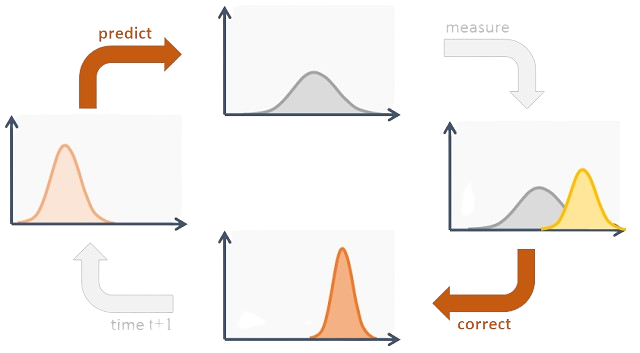
\includegraphics[width=\textwidth]{../../Images/Étapes du filtre de Kalman avec images.png}

	\end{column}
	\begin{column}{0.61\textwidth}

		\begin{block}{Limitations}
			\begin{itemize}
			\item Loss of optimality under non-linear models
			\item Cannot handle non-Gaussian PDFs
			\item[$\Rightarrow$] Not suited for \ballbullet{3} and \ballbullet{4}
			\end{itemize}
		\end{block}

	\end{column}
\end{columns}

\end{frame}

\begin{frame}{Particle filtering}

\begin{block}{Sequential importance sampling (SIS)}
	\begin{itemize}
	\item Asymptotically optimal under mild assumptions:
	\begin{itemize}
		\item $f_k$, $h_k$, $p(\eta_k)$ and $p(\varepsilon_k)$ known
	\end{itemize}
	\item Approximation of the posterior density by a mixture of Dirac distributions:
	\begin{equation}
		p(x_k\mid\mathbf{z}_{1:k})\:dx_k\approx\sum_{i=1}^Nw_k^{(i)}\:\delta_{x_k^{(i)}}(dx_k)
	\end{equation}
	\item Prediction step:
	\begin{equation}
		x_k^{(i)}\sim q\left(\cdot\:\middle|\:\mathbf{x}_{0:k-1}^{(i)},\mathbf{z}_{1:k}\right)=p\left(\cdot\:\middle|\:x_{k-1}^{(i)}\right)
	\end{equation}
	\item Correction step:
	\begin{equation}
		w_k^{(i)}\propto w_{k-1}^{(i)}\:\frac{\overbrace{p\left(z_k\:\middle|\:x_k^{(i)}\right)}^{\text{requires }h_k\text{\rlap{ so cannot be applied to {\ballbullet{5}} or \ballbullet{6}}}}\:p\left(x_k^{(i)}\:\middle|\:x_{k-1}^{(i)}\right)}{q\left(x_k^{(i)}\:\middle|\:\mathbf{x}_{0:k-1}^{(i)},\mathbf{z}_{1:k}\right)}=w_{k-1}^{(i)}\:p\left(z_k\:\middle|\:x_k^{(i)}\right)
	\end{equation}
	\end{itemize}
\end{block}

\end{frame}

\begin{frame}{Regularised particle filter (RPF)}

\begin{block}{Weight degeneracy}
	\begin{itemize}
	\item Over time, the weight distribution concentrates
	\item Collapse of the particle set onto a single particle: \ballbullet{7}
	\item[$\Rightarrow$] Particles resampled when effective sample size below threshold:
	\begin{equation}
		\textstyle\hat{N}_{\mathrm{eff}}\triangleq\left.1\middle/\sum_{i=1}^N\left(w_k^{(i)}\right)^2\right.<N_{\mathrm{th}}
	\end{equation}
	\end{itemize}
\end{block}

\begin{block}{Particle impoverishment}
	\begin{itemize}
		\item Resampled particles are copies of their parents
		\item Loss of particle diversity and exploration power: \ballbullet{8}
		\item[$\Rightarrow$] Regularisation by kernel density approximation of the PDF:
		\begin{equation}
			\textstyle p(x_k\mid\mathbf{z}_{1:k})\approx\sum_{i=1}^Nw_k^{(i)}\:K_\ell\left(x_k-x_k^{(i)}\right)
		\end{equation}
	\end{itemize}
\end{block}

\begin{columns}[onlytextwidth]
	\begin{column}{0.48\textwidth}

		\centering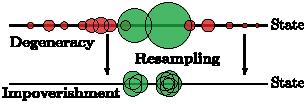
\includegraphics[width=\textwidth]{Images/Appauvrissement particulaire.pdf}

	\end{column}
	\begin{column}{0.48\textwidth}

		\centering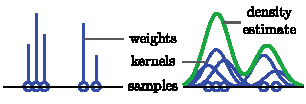
\includegraphics[width=\textwidth]{Images/Régularisation par noyau.pdf}

	\end{column}
\end{columns}

\end{frame}

\section{Gaussian processes}

\begin{frame}{Gaussian process regression}

\begin{block}{Unknown observation function}
	\begin{itemize}
		\item Bayesian correction is impossible in poorly known environment (\ballbullet{5})
		\item Multi-linear interpolation ignores data correlations and uncertainty
		\item[$\Rightarrow$] Kriging: analytical expression of $h_k$ and uncertainty, conditioned on $(\tilde{\mathbf{x}},\tilde{\mathbf{z}})$
	\end{itemize}
\end{block}

\begin{columns}[onlytextwidth]
	\begin{column}{0.6\textwidth}

		\begin{block}{Kernel hyperparameters}
			\begin{itemize}
				\item Known kernel form:
				\begin{equation}
					\hspace{-5mm}\kappa_{\frac{3}{2}}(r)=\sigma_h^2\left(1+\frac{\sqrt{3}r}{\ell}\right)\exp\left(-\frac{\sqrt{3}r}{\ell}\right)
				\end{equation}
				\item But unknown hyperparameters (HPs): \ballbullet{9}
				\item[$\Rightarrow$] Maximum likelihood estimation on $(\tilde{\mathbf{x}},\tilde{\mathbf{z}})$
			\end{itemize}
		\end{block}

	\end{column}
	\begin{column}{0.37\textwidth}

		\vspace{3mm}
		\centering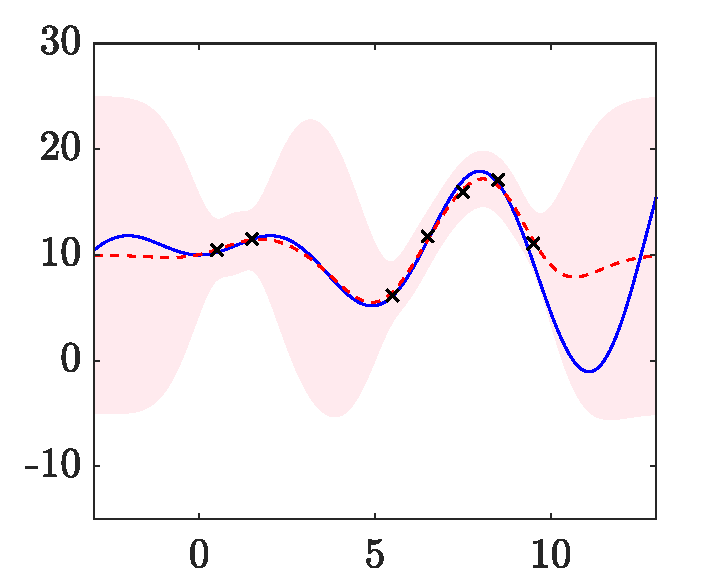
\includegraphics[width=\textwidth]{../../Images/Exemple de krigeage simple 2D.pdf}

	\end{column}
\end{columns}

\end{frame}

\begin{frame}{Simple kriging}

\begin{block}{Assumptions}
	\begin{itemize}
		\item Gaussian prior on the field, $h_k\sim\mathcal{GP}(m,\kappa)$:
		\begin{equation}
			\left\{\begin{aligned}
			z_k&=h_k(x_k)+\varepsilon_k\sim\mathcal{N}\Big(m(x_k),\kappa(x_k,x_k)+\mathbf{R}\Big)\\
			\forall i\in[\![1,\tilde{N}]\!],\:\tilde{z}_i&=h_k(\tilde{x}_i)+\tilde{\varepsilon}_i\sim\mathcal{N}\Big(m(\tilde{x}_i),\kappa(\tilde{x}_i,\tilde{x}_i)+\tilde{\mathbf{R}}\Big)
			\end{aligned}\right.
		\end{equation}
	\end{itemize}
\end{block}

\begin{block}{Gaussian process regression}
	\begin{itemize}
		\item Best linear unbiased estimator of $z$ given $\tilde{\mathbf{z}}$:
		\begin{equation}
			\left\{\begin{aligned}
			\hat{z}_{\mathrm{SK}}(x_k,\tilde{\mathbf{x}},\tilde{\mathbf{z}},m)&=\overbrace{m(x_k)}^{\text{prior}}+\overbrace{\kappa(x_k,\tilde{\mathbf{x}})\:\mathbf{G}(\tilde{\mathbf{x}})^{-1}}^{\text{gain}}\:\overbrace{(\tilde{\mathbf{z}}-m(\tilde{\mathbf{x}}))}^{\text{innovation}}\\
			\mathbf{R}_{\mathrm{SK}}(x_k,\tilde{\mathbf{x}})&=\kappa(x_k,x_k)+\mathbf{R}-\kappa(x_k,\tilde{\mathbf{x}})\:\mathbf{G}(\tilde{\mathbf{x}})^{-1}\kappa\left(\tilde{\mathbf{x}},x_k\right)
			\end{aligned}\right.
		\end{equation}
		\item Gaussian conditioning interpretation:
		\begin{equation}
			z_k\mid\tilde{\mathbf{z}}\sim\mathcal{N}\left(\hat{z}_{\mathrm{SK}}(x_k,\tilde{\mathbf{x}},\tilde{\mathbf{z}},m),\mathbf{R}_{\mathrm{SK}}(x_k,\tilde{\mathbf{x}})\right)
		\end{equation}
		\item Since $h_k$ is unknown, so is $m$: \ballbullet{10}
	\end{itemize}
\end{block}

\end{frame}

\begin{frame}{Universal kriging}

\begin{block}{Mean estimation}
	\begin{itemize}
		\item Joint estimation of $z$ and $m$ using trend functions to account for \ballbullet{10}:
		\begin{equation}
			\textstyle m(x)=g(x)\:\boldsymbol{\gamma}=\sum_{i=1}^{r_{\mathrm{UK}}}g_i(x)\:\gamma_i
		\end{equation}
		\item Link with simple kriging:
		\begin{equation}
			\left\{\begin{aligned}
				\hat{z}_{\mathrm{UK}}(x_k,\tilde{\mathbf{x}},\tilde{\mathbf{z}},g)&=\hat{z}_{\mathrm{SK}}\left(x_k,\tilde{\mathbf{x}},\tilde{\mathbf{z}},g\:\hat{m}_{\mathrm{UK}}(\tilde{\mathbf{x}},\tilde{\mathbf{z}},g)\right)\\
				\mathbf{R}_{\mathrm{UK}}(x_k,\tilde{\mathbf{x}},g)&=\mathbf{R}_{\hat{m}_{\mathrm{UK}}}(x_k,\tilde{\mathbf{x}},g)+\mathbf{R}_{\mathrm{SK}}(x_k,\tilde{\mathbf{x}})
			\end{aligned}\right.
		\end{equation}
		\item Risk of overfitting the mean: \ballbullet{11}
		\item[$\Rightarrow$] Ordinary kriging (OK): constant mean estimator, $r_{\mathrm{UK}}=1$ and $g_1\equiv1$
	\end{itemize}
\end{block}

\begin{columns}[onlytextwidth]
	\begin{column}{0.48\textwidth}

		\centering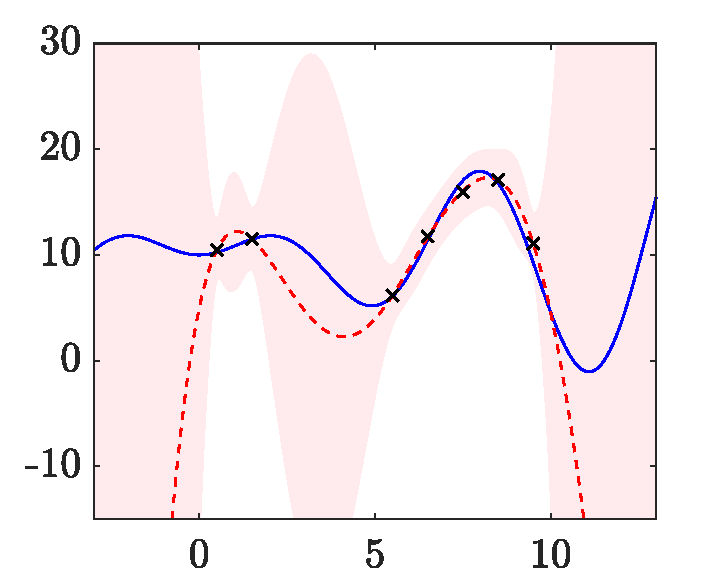
\includegraphics[width=0.8\textwidth]{../../Images/Exemple de krigeage universel à mauvaise base 2D.pdf}

	\end{column}
	\begin{column}{0.48\textwidth}

		\centering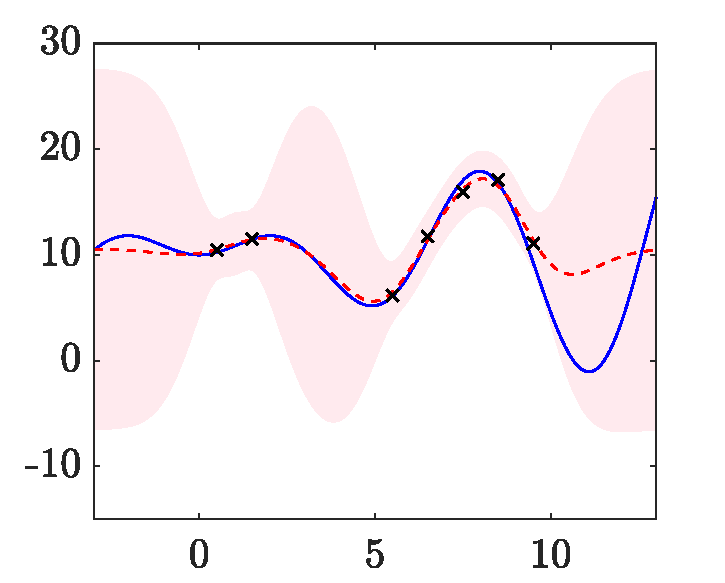
\includegraphics[width=0.8\textwidth]{../../Images/Exemple de krigeage ordinaire 2D.pdf}

	\end{column}
\end{columns}

\end{frame}

\section{Poorly known field}

\begin{frame}{Kriging-based particle filter}

\begin{block}{Kriging the observation model}
	\begin{itemize}
		\item If $\gamma_1\sim\mathcal{N}(0,\sigma^2)$ with $\sigma\rightarrow0$, then:
		\begin{equation}
			z_k\mid x_k,\tilde{\mathbf{z}}\sim\mathcal{N}\left(\hat{z}_{\mathrm{OK}}(x_k,\tilde{\mathbf{x}},\tilde{\mathbf{z}}),\:\mathbf{R}_{\mathrm{OK}}(x_k,\tilde{\mathbf{x}})\right)
		\end{equation}
		\item Naive approach: replace $h_k$ by $\hat{z}_{\mathrm{OK}}(\cdot,\tilde{\mathbf{x}},\tilde{\mathbf{z}})$ to solve \ballbullet{5}
	\end{itemize}
\end{block}

\centering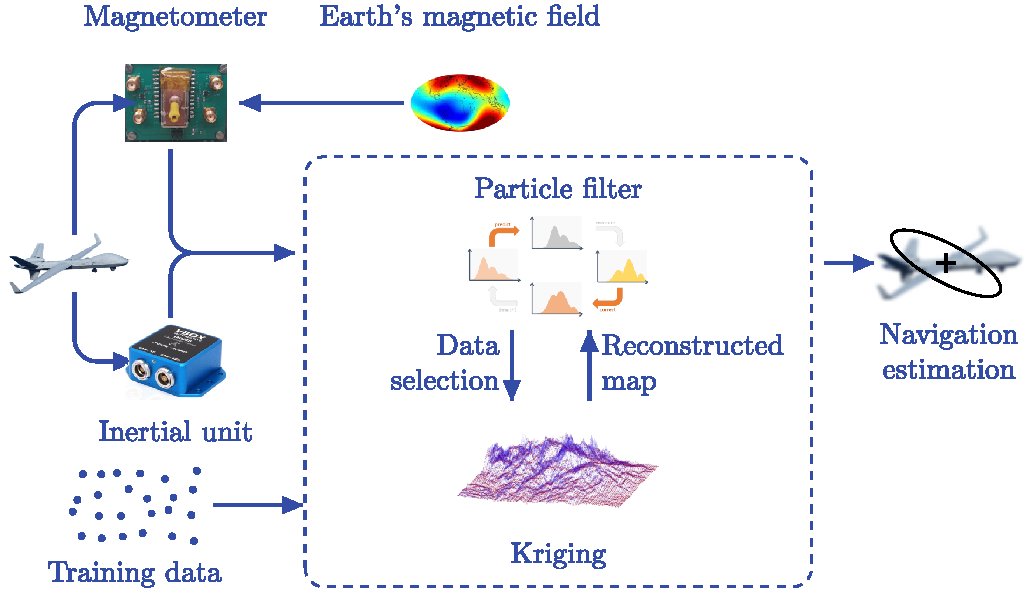
\includegraphics[width=0.8\textwidth]{../../Images/Schéma de l'application krigeage.pdf}

\end{frame}

\begin{frame}{Simulation scenario}

\begin{block}{Compared filters}
	\begin{itemize}
		\item Reference case: known map ($1$ km resolution)
		\item OK and bilinear interpolation for $6$ training sample resolutions
	\end{itemize}
\end{block}

\begin{columns}[onlytextwidth]
	\begin{column}{0.55\textwidth}

		\vspace{3mm}
		\centering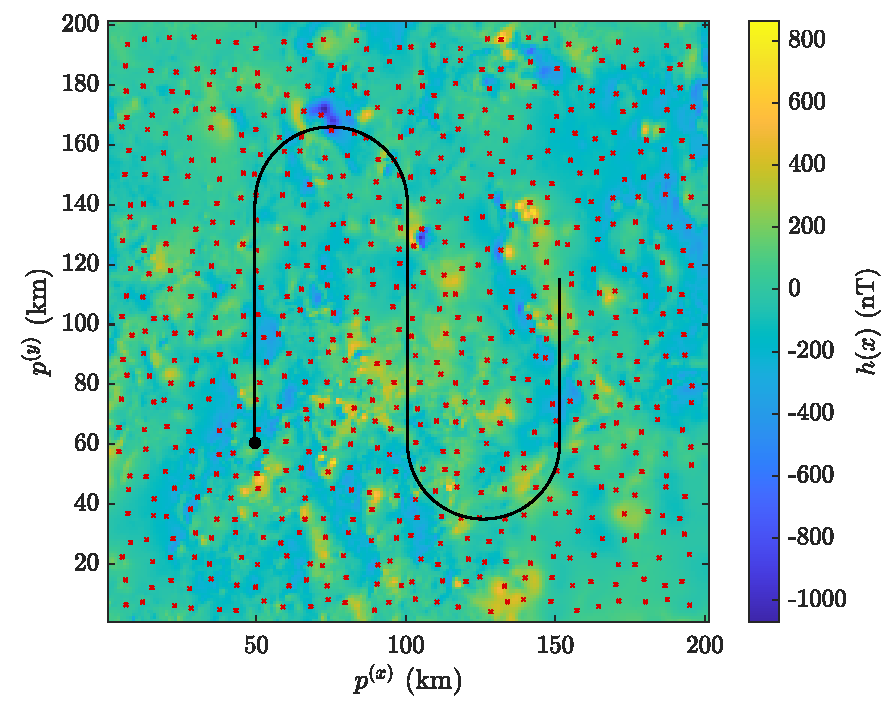
\includegraphics[width=\textwidth]{../../Images/Carte anomalie magnetique.pdf}

	\end{column}
	\begin{column}{0.43\textwidth}

		\centering\footnotesize
		\setlength{\tabcolsep}{2.5pt}
		\renewcommand{\arraystretch}{1.2}
		\begin{tabular}{|l|l|}\hline
			Sample resolution&$2.5$ to $7.5$ km\\
			Training points&$\in\{79^2,\dots,26^2\}$\\
			Training noise&$10^2$ $(\text{nT})^2$\\\hline
			UAV speed&$500$ m/s\\
			Time step&$5$ s\\
			Mission duration&$150$ steps\\
			Evolution noise&$100^2\text{ m}^2$, $1^2\text{ m}^2\text{s}^{-2}$\\
			Initial covariance&$8000^2\text{ m}^2$, $2^2\text{ m}^2\text{s}^{-2}$\\\hline
			Observation model&Kriging or bilinear\\
			Kriging kernel&Matérn, $\nu=3/2$\\
			Hyperparameters&Maximum likelihood\\
			Observation noise&$5^2$ $(\text{nT})^2$\\\hline
			Filter&RPF,$N=5000$\\
			Monte Carlo runs&$N_{\mathrm{MC}}=1000$\\\hline
		\end{tabular}

	\end{column}
\end{columns}

\end{frame}

\begin{frame}{Numerical results: accuracy and consistency}

\centering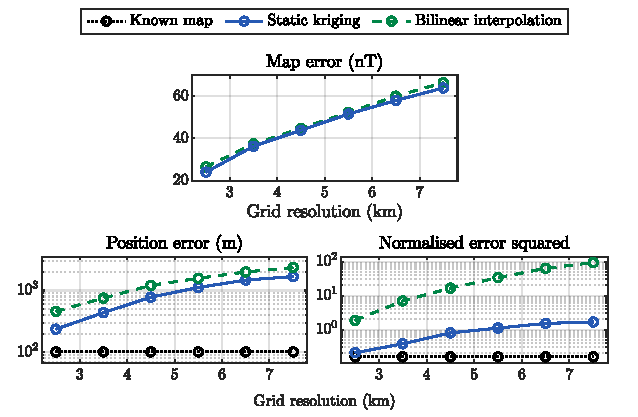
\includegraphics[width=\textwidth]{Images/Precision par maille.pdf}

\end{frame}

\begin{frame}{Numerical results: convergence and cost}

\centering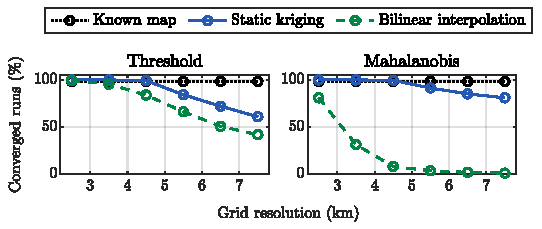
\includegraphics[width=0.85\textwidth]{Images/Convergence par maille.pdf}

\centering\footnotesize% Generated by figures_campagnes.m, do not edit by hand.
% Analytic flop counts per run, not timings, for 5000 particles over 150 steps.
% Setup solves the training system once; queries cost n^2 per particle and per
% step; total is their sum, the figure every comparison table of the chapter
% reports. The known map and bilinear interpolation are read in eight flops per
% query and pay no setup, hence one row each: neither depends on the map
% resolution.

\begin{tabular}{|l|ccc|c|}\hline
\multirow{2}{*}{Observation model} & \multicolumn{3}{c|}{Cost (flops)} & \multirow{2}{*}{Memory (bytes)}\\\cline{2-4}
 & Setup & Queries & Total & \\\hline
Known map & $0$ & $6$ M & $6$ M & $323$ k\\
Bilinear interpolation & $0$ & $6$ M & $6$ M & $150$ k\\\hline
Static kriging, $2.5$ km & $81$ G & $29.2$ T & $29.3$ T & $312$ M\\
Static kriging, $3.5$ km & $10.3$ G & $7.38$ T & $7.39$ T & $78.8$ M\\
Static kriging, $4.5$ km & $2.42$ G & $2.81$ T & $2.81$ T & $30$ M\\
Static kriging, $5.5$ km & $726$ M & $1.26$ T & $1.26$ T & $13.5$ M\\
Static kriging, $6.5$ km & $243$ M & $608$ G & $608$ G & $6.5$ M\\
Static kriging, $7.5$ km & $103$ M & $343$ G & $343$ G & $3.67$ M\\
\hline
\end{tabular}


\end{frame}

\section{Adaptive kriging}

\begin{frame}{Subsampled kriging}

\begin{block}{Limitations of static kriging}
	\begin{itemize}
		\item Heavy computational cost (between $0.46$ and $38.9$ Gflop/s): \ballbullet{12}
		\item Does not adapt to non-stationary fields (HPs and training data): \ballbullet{13}
	\end{itemize}
\end{block}

\begin{block}{Simple solution: random subsampling (RS)}
	\begin{itemize}
		\item Keeping each training point with probability $p_{\mathrm{RS}}=0.5$
		\item Solves \ballbullet{12} as is $4$ times cheaper
		\item But effective sample resolution reduced by $1/\sqrt{p_{\mathrm{RS}}}$
	\end{itemize}
\end{block}

\begin{block}{Requirements for the retained subset}
	\begin{itemize}
	\item Encompasses the particle set to avoid extrapolation
	\item Contains enough points to estimate the HPs
	\item Lies in a region small enough for the HPs to be constant
	\item Remains small enough for real-time computation
	\end{itemize}
\end{block}

\end{frame}

\begin{frame}{Adaptive kriging (AK)}

\begin{block}{Adaptive subsampling window}
	\begin{itemize}
		\item Ball centred on the predicted position, of radius $\max(r_{\mathrm{cov},k},r_{\min,k})$
		\item Coverage radius $r_{\mathrm{cov},k}$ to enclose $99\%$ of the particles, dilated by $\alpha_{\mathrm{AK}}=2$:
			\begin{equation}
				r_{\mathrm{cov},k}\triangleq\alpha_{\mathrm{AK}}\sqrt{\chi_{d_{\mathrm{pos}}}^2(99\%)}\sqrt{\lambda_{\max}\left(\hat{\mathbf{P}}_{\mathrm{pos},k|k-1}\right)}
			\end{equation}
		\item Minimum radius $r_{\min,k}$: at least $\tilde{N}_{\min}=25$ retained training points
		\item Hyperparameters re-estimated at each step on the window
		\item[$\Rightarrow$] Reduces the cost (\ballbullet{12}) and adapts to non-stationary fields (\ballbullet{13})
	\end{itemize}
\end{block}

\centering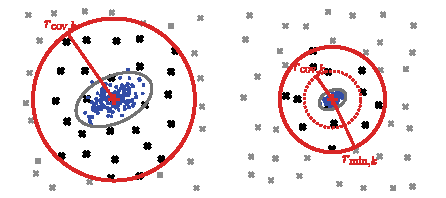
\includegraphics[width=0.7\textwidth]{Images/Construction de la fenêtre AK.pdf}

\end{frame}

\begin{frame}{Non-spherical subsampling windows}

\begin{block}{Macroscopic view}
	\begin{itemize}
	\item AK: one ball for the entire set, treats the PDF as Gaussian
	\item May not fully address \ballbullet{12} and \ballbullet{13} for multimodal distributions: \ballbullet{14}
	\end{itemize}
\end{block}

\begin{block}{Nearest neighbour adaptive kriging (NNAK)}
	\begin{itemize}
	\item Microscopic view: one ball per particle, $\tilde{N}_{\min}=10$ nearest training points
	\item Retained data: their union, which follows even a multimodal PDF (\ballbullet{14})
	\item HP estimation and kriging as for AK
	\end{itemize}
\end{block}

\begin{block}{A third scale}
	\begin{itemize}
	\item Two extremes: one ball for the whole set (AK) or one per particle (NNAK)
	\item A multimodal PDF can be split into unimodal parts, one per mode
	\item[$\Rightarrow$] Mesoscopic view left to explore, subsampling mode by mode: \ballbullet{15}
	\end{itemize}
\end{block}

\end{frame}

\begin{frame}{Clustered adaptive kriging (ICAK, MCAK)}

\begin{columns}[onlytextwidth]
	\begin{column}{0.61\textwidth}

		\begin{block}{Clustering the particle set}
			\begin{itemize}
			\item Number of clusters unknown and varying
			\item Mean shift: each particle climbs to a mode of the regularised PDF:
			\begin{equation}
				\frac{\partial p}{\partial x}(x)\propto\frac{\displaystyle\sum_{i\in\mathcal{B}(x,\ell)}w_k^{(i)}\:x_k^{(i)}}{\displaystyle\sum_{i\in\mathcal{B}(x,\ell)}w_k^{(i)}}-x
			\end{equation}
			\item Clusters as equivalence classes of the modes
			\end{itemize}
		\end{block}

	\end{column}
	\begin{column}{0.37\textwidth}

		\vspace{6mm}\hspace*{0mm}
		\centering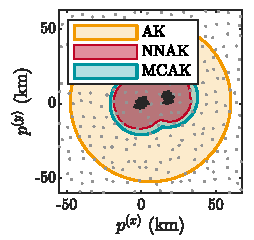
\includegraphics[width=\textwidth]{Images/Formes des fenetres.pdf}

	\end{column}
\end{columns}

\begin{block}{Independent or merged kriging}
	\begin{itemize}
	\item ICAK: one AK window per cluster, kriged separately with its own HPs
	\item MCAK: union of these windows, kriged as AK with a single HP estimation
	\item[$\Rightarrow$] MCAK reduces to AK (one cluster) and to NNAK (one cluster per particle)
	\end{itemize}
\end{block}

\end{frame}

\begin{frame}{Adaptive kriging: accuracy and consistency at $7.5$ km}

\begin{center}
	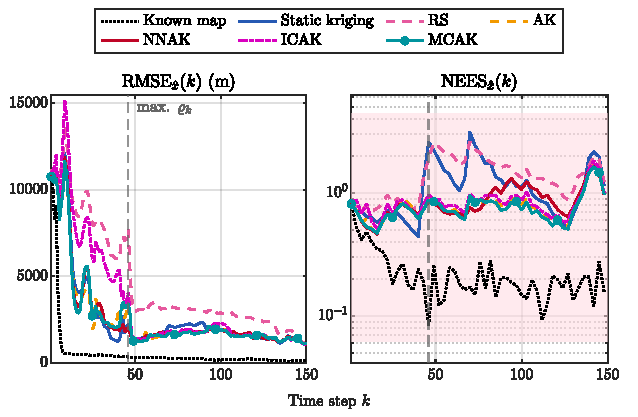
\includegraphics[width=\textwidth]{Images/RMSE et NEES sous-echantillonnage.pdf}
\end{center}

\end{frame}

\begin{frame}{Adaptive kriging: convergence and cost}

\centering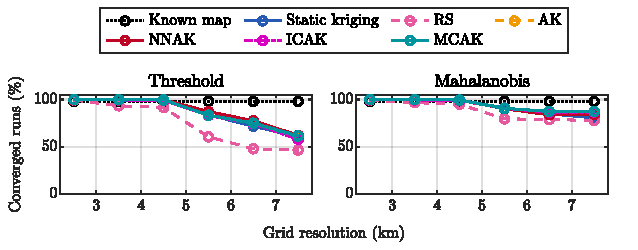
\includegraphics[width=\textwidth]{Images/Convergence sous-echantillonnage.pdf}

\makebox[\textwidth][c]{\footnotesize% Generated by figures_campagnes.m, do not edit by hand.
% Analytic flop counts per run, not timings, for 5000 particles over 150 steps:
% kriging (factorisation and queries), then for the adaptive methods the rest
% gathered, HP for the local hyperparameter fits plus the mean-shift of the
% ICAK and the MCAK (clust.) or the neighbour search of the NNAK (NN).

{\setlength{\tabcolsep}{2.5pt}%
\begin{tabular}{|c|c|c|cc|cc|cc|cc|}\hline
\multirow{2}{*}{$\Delta_g$} & \multirow{2}{*}{\shortstack{Static\\kriging}} & \multirow{2}{*}{\shortstack{RS}} & \multicolumn{2}{c|}{AK} & \multicolumn{2}{c|}{NNAK} & \multicolumn{2}{c|}{ICAK} & \multicolumn{2}{c|}{MCAK}\\\cline{4-5}\cline{6-7}\cline{8-9}\cline{10-11}
 & & & Kriging & HP & Kriging & HP + NN & Kriging & HP + clust. & Kriging & HP + clust.\\\hline
$2.5$ km & $29.3$ T & $7.3$ T & $46$ G & $564$ M & $4.3$ G & $104$ M & $2.26$ G & $201$ M & $24.3$ G & $453$ M\\
$3.5$ km & $7.39$ T & $1.84$ T & $14.4$ G & $224$ M & $2.05$ G & $79.6$ M & $901$ M & $241$ M & $7.61$ G & $308$ M\\
$4.5$ km & $2.81$ T & $704$ G & $5.75$ G & $121$ M & $1.23$ G & $66.8$ M & $616$ M & $277$ M & $3.5$ G & $292$ M\\
$5.5$ km & $1.26$ T & $314$ G & $3.09$ G & $89.8$ M & $885$ M & $60.5$ M & $547$ M & $314$ M & $2.12$ G & $300$ M\\
$6.5$ km & $608$ G & $152$ G & $1.93$ G & $70.1$ M & $705$ M & $56.2$ M & $513$ M & $357$ M & $1.54$ G & $319$ M\\
$7.5$ km & $343$ G & $85.9$ G & $1.54$ G & $66.7$ M & $603$ M & $53.4$ M & $499$ M & $401$ M & $1.25$ G & $337$ M\\
\hline
\end{tabular}
}
}

\end{frame}

\begin{frame}{Errors of the kriged observation model}

\textbf{TODO: reprendre ici}

\begin{block}{Map errors}
	\begin{itemize}
	\item Innovation:\hfill$z_k-\hat{z}_{\mathrm{UK}}(x_k,\tilde{\mathbf{x}},\tilde{\mathbf{z}})=\zeta_h(x_k)+\zeta_\varepsilon(x_k)+\varepsilon_k$\hfill\stepcounter{equation}(\theequation)
	\item Kriging error from noise-free training data:\hfill$\zeta_h(x)=h(x)-\hat{z}_{\mathrm{UK}}\left(x,\tilde{\mathbf{x}},h(\tilde{\mathbf{x}})\right)$
	\item Effect of the training noise:\hfill$\zeta_\varepsilon(x)=\hat{z}_{\mathrm{UK}}\left(x,\tilde{\mathbf{x}},h(\tilde{\mathbf{x}})\right)-\hat{z}_{\mathrm{UK}}(x,\tilde{\mathbf{x}},\tilde{\mathbf{z}})$
	\item Unlike $\varepsilon_k$, fixed during the mission: correlated along the trajectory
	\end{itemize}
\end{block}

\begin{block}{Subsampling errors}
	\begin{itemize}
	\item Survey split into retained and discarded points: $\tilde{\mathbf{x}}=(\tilde{\mathbf{x}}^r,\tilde{\mathbf{x}}^d)$
	\item Kriging from the retained points alone adds a fourth term:
	\begin{equation}
		\begin{aligned}
		z_k-\hat{z}_{\mathrm{UK}}(x_k,\tilde{\mathbf{x}}^r,\tilde{\mathbf{z}}^r)&=\zeta_h(x_k)+\zeta_\varepsilon(x_k)+\varepsilon_k\\
		&\quad+\hat{z}_{\mathrm{UK}}(x_k,\tilde{\mathbf{x}},\tilde{\mathbf{z}})-\hat{z}_{\mathrm{UK}}(x_k,\tilde{\mathbf{x}}^r,\tilde{\mathbf{z}}^r)
		\end{aligned}
	\end{equation}
	\item Interpolation error $\zeta_{\hat{z}}$: norm of this term
	\item Subsampling error covariance $\zeta_{\mathbf{R}}$: its covariance, with $\sigma_{\mathbf{R}}=\sqrt{\lambda_{\max}(\zeta_{\mathbf{R}})}$
	\end{itemize}
\end{block}

\end{frame}

\begin{frame}{Guarantees on the subsampling error}

\begin{block}{Kalman-like correction by the discarded data}
	\begin{itemize}
	\item\hfill$\hat{z}_{\mathrm{UK}}(x,\tilde{\mathbf{x}},\tilde{\mathbf{z}})=\hat{z}_{\mathrm{UK}}(x,\tilde{\mathbf{x}}^r,\tilde{\mathbf{z}}^r)+\underbrace{\kappa_{d|r}(x)^\top\mathbf{S}_{d|r}^{-1}}_{\text{gain}}\:\underbrace{\tilde{\mathbf{z}}_{d|r}}_{\text{innovation}}$\hfill\stepcounter{equation}(\theequation)
	\item $\tilde{\mathbf{z}}_{d|r}\sim\mathcal{N}(0,\mathbf{S}_{d|r})$: discarded data minus their prediction from the retained data, and $\kappa_{d|r}(x)$ their residual covariance with $x$
	\end{itemize}
\end{block}

\begin{block}{Covariance inflation and error bounds}
	\begin{itemize}
	\item\hfill$\zeta_{\mathbf{R}}(x)=\mathbf{R}_{\mathrm{UK}}(x,\tilde{\mathbf{x}}^r)-\mathbf{R}_{\mathrm{UK}}(x,\tilde{\mathbf{x}})\succeq0$\hfill\stepcounter{equation}(\theequation)
	\item[$\Rightarrow$] Reported covariance inflated by exactly $\zeta_{\mathbf{R}}$: not overconfident
	\item Bound from the retained data alone:\hfill$\sigma_{\mathbf{R}}(x)^2\leq\lambda_{\max}\left(\mathbf{R}_{\mathrm{UK}}(x,\tilde{\mathbf{x}}^r)-\mathbf{R}\right)$\hfill\stepcounter{equation}(\theequation)
	\item With probability at least $1-\delta$:\hfill$\zeta_{\hat{z}}(x)\leq\sqrt{\chi^2_{d_z}(1-\delta)}\:\sigma_{\mathbf{R}}(x)$\hfill\stepcounter{equation}(\theequation)
	\item For every realisation, even with a misspecified GP:\\
	\hfill$\zeta_{\hat{z}}(x)\leq\sigma_{\mathbf{R}}(x)\:\|\tilde{\mathbf{z}}_{d|r}\|_{\mathbf{S}_{d|r}}$\hfill\stepcounter{equation}(\theequation)
	\end{itemize}
\end{block}

\end{frame}

\begin{frame}
\pgfdeclarelayer{fond}
\pgfsetlayers{fond,main}
\begin{tikzpicture}[
	x=2.25cm, y=-1.4cm,
	methode/.style={draw=structure.fg, fill=structure.fg!8, rounded corners=2pt, text width=1.7cm, minimum height=8mm, align=center, inner sep=1pt, font=\small},
	fleche/.style={-stealth, thick, structure.fg},
	enjeu/.style={circle, shade, shading=ball, ball color=structure.fg, text=white, inner sep=0pt, minimum size=2.2ex},
	groupe/.style={draw=structure.fg!60, densely dashed, rounded corners=4pt, overlay},
	contribution/.style={draw=structure.fg, thick, fill=structure.fg!18, rounded corners=4pt, overlay},
]
	% Navigation
	\node[methode] (auto) at (0,0) {Autonomous navigation};
	\node[methode] (ins)  at (0,1) {Inertial navigation};
	\node[methode] (bay)  at (1,1) {Bayesian estimation};
	\node[methode] (gnss) at (1,2) {GNSS navigation};
	\node[methode] (fan)  at (2,2) {Field-aided navigation};
	% Filtrage
	\node[methode] (kf)   at (1,0) {Kalman filter};
	\node[methode] (sis)  at (2,0) {SIS};
	\node[methode] (pf)   at (3,0) {Generic PF};
	\node[methode] (rpf)  at (4,0) {RPF};
	% Krigeage
	\node[methode] (hp)   at (3,2) {HP\\estimation};
	\node[methode] (sk)   at (3,1) {(Simple) kriging};
	\node[methode] (uk)   at (4,1) {Universal kriging};
	\node[methode] (ok)   at (4,2) {Ordinary kriging};
	% Krigeage adaptatif
	\node[methode] (kpf)  at (4,3) {Kriging-based RPF};
	\node[methode] (rs)   at (4,4) {(Random) subsampling};
	\node[methode] (ak)   at (3,4) {AK-RPF};
	\node[methode] (nnak) at (3,3) {NNAK-RPF};
	\node[methode] (cak)  at (3,5) {ICAK-RPF MCAK-RPF};
	\node[methode] (sub)  at (4,5) {Error bounds};

	% Groupes, tracés avant les flèches qui les traversent
	\draw[groupe] ([xshift=-3pt, yshift=-3pt]kf.south west) rectangle ([xshift=3pt, yshift=3pt]rpf.north east);
	\draw[groupe] ([xshift=-3pt, yshift=-3pt]hp.south west) rectangle ([xshift=3pt, yshift=3pt]uk.north east);
	\begin{pgfonlayer}{fond}
		\draw[contribution] ([xshift=-3pt, yshift=-3pt]cak.south west) rectangle ([xshift=3pt, yshift=3pt]kpf.north east);
	\end{pgfonlayer}

	\draw[fleche] (auto) -- (ins);
	\draw[fleche] (ins)  -- node[enjeu, above=1pt] {\scalebox{0.8}{1}} (bay);
	\draw[fleche] (bay)  -- (gnss);
	\draw[fleche] (gnss) -- node[enjeu, above=1pt] {\scalebox{0.8}{2}} (fan);
	\draw[fleche] (bay)  -- (kf);
	\draw[fleche] (kf)   -- node[enjeu, above=1pt] {\scalebox{0.8}{3}} (sis);
	\draw[fleche] ([xshift=-10pt]fan.north) -- node[enjeu, left=1pt] {\scalebox{0.8}{4}} ([xshift=-10pt]sis.south);
	\draw[fleche] (sis)  -- node[enjeu, above=1pt] {\scalebox{0.8}{7}} (pf);
	\draw[fleche] (pf)   -- node[enjeu, above=1pt] {\scalebox{0.8}{8}} (rpf);
	\draw[fleche, rounded corners=2pt] ([xshift=10pt]fan.north) |- node[enjeu, above=1pt, pos=0.75] {\scalebox{0.8}{5}} (sk.west);
	\draw[fleche] (sk)   -- node[enjeu, right=1pt] {\scalebox{0.8}{9}} (hp);
	\draw[fleche] (sk)   -- node[enjeu, above=1pt] {\scalebox{0.8}{10}} (uk);
	\draw[fleche] (uk)   -- node[enjeu, right=1pt] {\scalebox{0.8}{11}} (ok);
	\draw[fleche] (ok)   -- (kpf);
	\draw[fleche, overlay, rounded corners=2pt] (rpf.east) -- ++(10pt,0) |- (kpf.east);
	\draw[fleche] (kpf)  -- node[enjeu, right=1pt] {\scalebox{0.8}{12}} (rs);
	\draw[fleche] (rs)   -- node[enjeu, right=1pt] {\scalebox{0.8}{16}} (sub);
	\draw[fleche] (rs)   -- node[enjeu, above=1pt] {\scalebox{0.8}{13}} (ak);
	\draw[fleche] (ak)   -- node[enjeu, right=1pt] {\scalebox{0.8}{14}} (nnak);
	\draw[fleche] (ak)   -- node[enjeu, right=1pt] {\scalebox{0.8}{15}} (cak);
\end{tikzpicture}

\end{frame}

\end{document}

\section{Unknown field}

\begin{frame}{Navigation over an unknown field}

\begin{block}{Simultaneous localisation and mapping (SLAM)}
	\begin{itemize}
	\item No survey: $h$ is learnt from the observations of the vehicle itself
	\item Each observation is taken at an uncertain position
	\item Assumption: $h\sim\mathcal{GP}(0,\kappa_\nu)$, stationary, with known hyperparameters
	\end{itemize}
\end{block}

\begin{block}{Requirements}
	\begin{itemize}
	\item Recursive: no growing history of observations
	\item Finite-dimensional map, with $r$ basis functions $\boldsymbol{\Psi}=(\psi_1,\dots,\psi_r)$:\\
	\hfill$h(x)\approx\boldsymbol{\Psi}(x)\:\boldsymbol{\gamma},\qquad\boldsymbol{\gamma}\in\mathbb{R}^r$\hfill(17)
	\item Joint estimation of the state $x_k$ and of the coefficients $\boldsymbol{\gamma}$
	\end{itemize}
\end{block}

\end{frame}

\begin{frame}{State of the art: RBPF-SLAM}

\begin{block}{Rao-Blackwellised PF with a reduced-rank GP map \source{Kok \& Solin, FUSION 2018}}
	\begin{itemize}
	\item Laplace eigenfunctions on a domain $\Omega$ \source{Solin \& Särkkä, 2020}: $\boldsymbol{\gamma}\sim\mathcal{N}(0,\boldsymbol{\Lambda})$, rank $r_{\mathrm{KL}}$
	\item Given the trajectory of a particle, $\boldsymbol{\gamma}$ is Gaussian $\rightarrow$ one Kalman filter per particle, weighted by its innovation
	\item Originally for the 3D magnetic field over tiled domains; here a scalar field over a single domain
	\end{itemize}
\end{block}

\begin{block}{Properties}
	\begin{itemize}
	\item Cost and memory in $\mathcal{O}(N\:r_{\mathrm{KL}}^2)$: one $r_{\mathrm{KL}}\times r_{\mathrm{KL}}$ covariance matrix per particle
	\item Resampling duplicates the maps: known degeneracy over time \source{Bailey et al., ICRA 2006}
	\item The basis must resolve the shortest wavelength of the field over the whole of $\Omega$
	\end{itemize}
\end{block}

\end{frame}

\begin{frame}{Filtering in a reproducing kernel Hilbert space (RKHS)}

\begin{block}{Kernel mean embedding}
	\begin{itemize}
	\item A distribution is represented by its mean in the RKHS of a kernel $\kappa_X$:\\
	\hfill$\displaystyle\mu_k\approx\sum_{i=1}^Nw_k^{(i)}\:\kappa_X\left(x_k^{(i)},\cdot\right)$\hfill(18)
	\item Expectations and conditioning become linear operations in this space
	\end{itemize}
\end{block}

\begin{block}{Adaptive kernel Kalman filter (AKKF) \source{Sun et al., IEEE TSP 2023}}
	\begin{itemize}
	\item Particles propagated as in a PF; weights $\mathbf{w}_k$ and their covariance $\boldsymbol{\Sigma}_k$ updated by a Kalman-like recursion:\\
	\hfill$\mathbf{w}_k=\mathbf{w}_{k-1}^++\mathbf{K}_k\left(\kappa_Z(\mathbf{z}_k,z_k)-\mathbf{G}_k^Z\:\mathbf{w}_{k-1}^+\right)$\hfill(19)
	\item $\mathbf{z}_k$: observations simulated at the particles, $z_k^{(i)}=h\left(x_k^{(i)}\right)+\varepsilon_k^{(i)}$
	\item[$\Rightarrow$] Requires $h$
	\item New particles drawn from $\mathcal{N}(\hat{x}_k,\hat{\mathbf{P}}_k)$ at each step
	\end{itemize}
\end{block}

\end{frame}

\begin{frame}{Learning the map: random features and recursive least squares}

\begin{block}{Random Fourier features (RFF) \source{Rahimi \& Recht, NeurIPS 2007}}
	\begin{itemize}
	\item Bochner: a stationary kernel is the Fourier transform of a spectral density
	\item Monte Carlo over $r_{\mathrm{RFF}}$ random frequencies $\omega_j$ and phases $b_j$:\\
	\hfill$\kappa_\nu(x,x')\approx\sigma_h^2\:\boldsymbol{\Psi}(x)\:\boldsymbol{\Psi}(x')^\top,\qquad\psi_j(x)=\sqrt{\tfrac{2}{r_{\mathrm{RFF}}}}\cos\left(\omega_j^\top x+b_j\right)$\hfill(20)
	\item Basis defined on the whole plane: no domain to choose
	\end{itemize}
\end{block}

\begin{block}{Recursive least squares (RLS)}
	\begin{itemize}
	\item One coefficient vector for all particles, fitted on the pairs $(\hat{x}_l,z_l)$:\\
	\hfill$\displaystyle J_k(\boldsymbol{\gamma})=\sum_{l=1}^k\beta_{\mathrm{RLS}}^{k-l}\left(z_l-\boldsymbol{\Psi}(\hat{x}_l)\:\boldsymbol{\gamma}\right)^2+\beta_{\mathrm{RLS}}^k\alpha_{\mathrm{RLS}}\|\boldsymbol{\gamma}\|_2^2$\hfill(21)
	\item Kalman-like update in $\mathcal{O}(r_{\mathrm{RFF}}^2)$: fixed cost, no stored history
	\end{itemize}
\end{block}

\end{frame}

\begin{frame}{AKKF-SLAM}

\begin{block}{One iteration}
\begin{algorithmic}\setstretch{1.15}
	\State{$\forall i,\:x_k^{(i)}\sim p\left(\cdot\:\middle|\:x_{k-1}^{+(i)}\right)$}\Comment{Prediction}
	\State{\textcolor{BrickRed}{$\forall i,\:z_k^{(i)}=\boldsymbol{\Psi}\left(x_k^{(i)}\right)\hat{\boldsymbol{\gamma}}_{k-1}+\varepsilon_k^{(i)}$}}\Comment{\textcolor{BrickRed}{Simulated observations}}
	\State{$\mathbf{w}_k=\mathbf{w}_{k-1}^++\mathbf{K}_k\left(\kappa_Z(\mathbf{z}_k,z_k)-\mathbf{G}_k^Z\:\mathbf{w}_{k-1}^+\right)$}\Comment{Embedded correction}
	\State{$\hat{x}_k$ and $\hat{\mathbf{P}}_k$ from $\mathbf{w}_k$ and $\boldsymbol{\Sigma}_{k|k}$}\Comment{State estimation}
	\State{\textcolor{BrickRed}{$\hat{\boldsymbol{\gamma}}_k=\hat{\boldsymbol{\gamma}}_{k-1}+\mathbf{K}_k^\gamma\left(z_k-\boldsymbol{\Psi}(\hat{x}_k)\:\hat{\boldsymbol{\gamma}}_{k-1}\right)$}}\Comment{\textcolor{BrickRed}{Map update (RLS)}}
	\State{$\forall i,\:x_k^{+(i)}\sim\mathcal{N}\left(\hat{x}_k,\hat{\mathbf{P}}_k\right)$}\Comment{Resampling}
\end{algorithmic}
\end{block}

\begin{block}{Properties}
	\begin{itemize}
	\item Simulated observations carry the map uncertainty: variance $\mathbf{R}_k\left(1+\boldsymbol{\Psi}\:\mathbf{P}_{k-1}^\gamma\:\boldsymbol{\Psi}^\top\right)$
	\item One map for all particles: memory in $\mathcal{O}(N^2+r_{\mathrm{RFF}}^2)$, cost in $\mathcal{O}(N^3+N\:r_{\mathrm{RFF}}^2)$ per step
	\item The map is learnt at the estimated positions, whose uncertainty is ignored
	\end{itemize}
\end{block}

\end{frame}

\begin{frame}{SLAM scenario}

\begin{columns}[onlytextwidth,T]
\begin{column}{0.47\textwidth}

\centering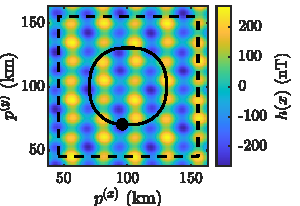
\includegraphics[width=\textwidth]{Images/Champ et circuit du SLAM.pdf}

\end{column}
\begin{column}{0.5\textwidth}

\begin{block}{Field and mission}
	\begin{itemize}
	\item Analytical field with three spatial frequencies, shortest wavelength $15$ km, standard deviation $123$ nT
	\item Closed circuit of $196$ km, flown $3.8$ times in $300$ steps
	\item Initial uncertainty of $1$ km per axis, which no SLAM can correct
	\item No survey
	\end{itemize}
\end{block}

\end{column}
\end{columns}

\begin{block}{Compared filters ($N=500$ particles, $100$ Monte Carlo runs)}
	\begin{itemize}
	\item References: RPF and AKKF on the known field, inertial navigation
	\item RBPF-SLAM with $r_{\mathrm{KL}}=300$ against AKKF-SLAM with $r_{\mathrm{RFF}}=500$
	\end{itemize}
\end{block}

\end{frame}

\begin{frame}{SLAM: position error and consistency}

\begin{columns}[onlytextwidth]
\begin{column}{0.5\textwidth}

\centering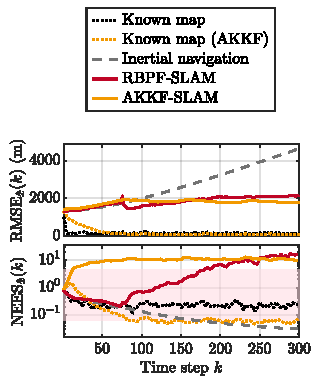
\includegraphics[width=\textwidth]{Images/RMSE et NEES du SLAM.pdf}

\end{column}
\begin{column}{0.47\textwidth}

\begin{block}{Position error (ARMSE)}
	\begin{itemize}
	\item Inertial navigation: $2.7$ km
	\item RBPF-SLAM: $1.82$ km
	\item AKKF-SLAM: $1.78$ km, flat after the first lap
	\item Runs ending below $2$ km: $73\%$ (AKKF), $50\%$ (RBPF)
	\end{itemize}
\end{block}

\begin{block}{Consistency (NEES)}
	\begin{itemize}
	\item RBPF-SLAM: leaves the band at $k=179$ (map degeneracy)
	\item AKKF-SLAM: $10$--$14$, constant, due to the learnt map
	\end{itemize}
\end{block}

\end{column}
\end{columns}

\end{frame}

\begin{frame}{SLAM: reconstructed field}

\begin{columns}[onlytextwidth]
\begin{column}{0.56\textwidth}

\centering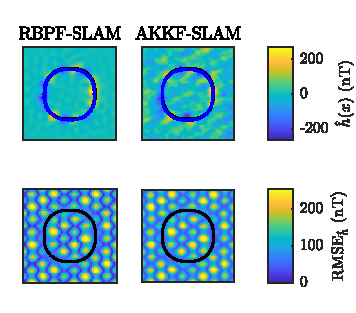
\includegraphics[width=\textwidth]{Images/Cartes reconstruites du SLAM.pdf}

\end{column}
\begin{column}{0.41\textwidth}

\begin{block}{Field error along the circuit}
	\begin{itemize}
	\item No map: $102.5$ nT
	\item RBPF-SLAM: $78.9$ nT
	\item AKKF-SLAM: $79.8$ nT
	\end{itemize}
\end{block}

\begin{block}{Limits}
	\begin{itemize}
	\item Field recovered only near the circuit
	\item A position error of about $2$ km is transferred to a field whose shortest wavelength is $15$ km
	\end{itemize}
\end{block}

\end{column}
\end{columns}

\end{frame}

\begin{frame}{SLAM: cost and rank of the basis}

\begin{columns}[onlytextwidth]
\begin{column}{0.47\textwidth}

\centering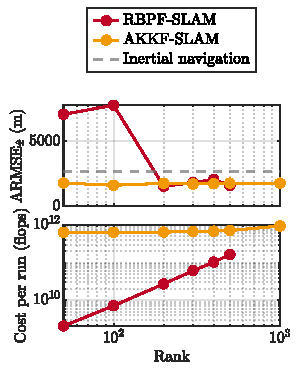
\includegraphics[width=\textwidth]{Images/Rangs du SLAM.pdf}

\end{column}
\begin{column}{0.5\textwidth}

\begin{block}{Cost per run}
	\begin{itemize}
	\item RBPF-SLAM: $60.9$ Gflop, $361$ MB
	\item AKKF-SLAM: $713$ Gflop, $8$ MB
	\item[$\Rightarrow$] $45$ times less memory, $12$ times more operations
	\item At equal cost, RBPF-SLAM is more accurate
	\end{itemize}
\end{block}

\begin{block}{Rank of the basis}
	\begin{itemize}
	\item RBPF-SLAM diverges for $r_{\mathrm{KL}}\leq100$, too coarse for the $15$ km wavelength
	\item AKKF-SLAM: $1.6$--$1.8$ km for any $r_{\mathrm{RFF}}$ from $50$ to $1000$
	\end{itemize}
\end{block}

\end{column}
\end{columns}

\end{frame}

\section{Conclusion}

\begin{frame}{Conclusion}

\begin{block}{\ballbulletinv{1} Representing the field by a GP}
	\begin{itemize}
	\item Kriging gives the map and its uncertainty: final error $1.4$ to $1.9$ times lower than bilinear interpolation, consistent NEES
	\item Subsampling error: exact decomposition, bounded, never overconfident
	\end{itemize}
\end{block}

\begin{block}{\ballbulletinv{2} Navigating over a poorly known field}
	\begin{itemize}
	\item Adaptive kriging: same accuracy, $213$ to $629$ times cheaper
	\item Clustering only helps multimodal particle sets
	\end{itemize}
\end{block}

\begin{block}{\ballbulletinv{3} Navigating over an unknown field}
	\begin{itemize}
	\item AKKF-SLAM: a single RFF map, learnt by RLS and shared by all particles
	\item As accurate as RBPF-SLAM: $45$ times less memory, $12$ times more flops
	\end{itemize}
\end{block}

\end{frame}

\begin{frame}{Perspectives}

\begin{block}{Towards real missions}
	\begin{itemize}
	\item Real data: sensor biases, which an RBPF could estimate, and time-varying fields
	\item Fusion of several physical fields, quantified by the Fisher information
	\end{itemize}
\end{block}

\begin{block}{Field representation}
	\begin{itemize}
	\item Spatially varying hyperparameters instead of local stationarity
	\item Uncertainty of the training inputs, for the survey and for SLAM
	\item Subsampling bounds that avoid inverting $\mathbf{S}_{d|r}$
	\end{itemize}
\end{block}

\begin{block}{SLAM}
	\begin{itemize}
	\item Start from a kriged region, which makes the initial position observable
	\item Loop closures; overlapping tiles, or forgetting distant data with $\beta_{\mathrm{RLS}}$
	\end{itemize}
\end{block}

\end{frame}

\begin{frame}{Publications}

\begin{block}{International conferences}
	\begin{itemize}\setlength\itemsep{2mm}
	\item B. Hubert, K. Dahia, N. Merlinge, A. Giremus, \emph{Adaptive Kriging Particle Filter and its Application to Terrain-Aided Navigation}, FUSION 2024
	\item B. Hubert, K. Dahia, N. Merlinge, A. Giremus, \emph{A Clustered Approach to Adaptive Kriging Particle Filter for Magnetic Field-Aided Navigation}, EUSIPCO 2025
	\item B. Hubert, K. Dahia, N. Merlinge, A. Giremus, \emph{Learning Observation Model for SLAM via Random Fourier Features in a Kernel Kalman Filter}, FUSION 2026
	\end{itemize}
\end{block}

\begin{block}{In preparation}
	\begin{itemize}
	\item Journal paper on the subsampling error bounds of kriging
	\end{itemize}
\end{block}

\end{frame}

\begin{frame}

\vspace{1cm}

\begin{beamercolorbox}[sep=8pt,center,rounded=true,shadow=true]{title}
	\usebeamerfont{title}Thank you for your attention
\end{beamercolorbox}

\vspace{5mm}

\begin{center}
	Questions?
\end{center}

\end{frame}

% Annexes : hors décompte, pour les questions du jury

\appendix
\miniframesoff
\section{Backup}

\begin{frame}{Backup: performance metrics}

\begin{block}{Position error and consistency}
	\begin{itemize}
	\item RMSE over the $N_{\mathrm{conv}}$ runs that converge under the threshold criterion (chapter 5: over all runs):\\
	\hfill$\displaystyle\mathrm{RMSE}_{\hat{x}}(k)=\sqrt{\frac{1}{N_{\mathrm{conv}}}\sum_{i\text{ convergent}}\left\|\boldsymbol{\Pi}_{\mathrm{pos}}\:\hat{x}_k^{(i)}-\boldsymbol{\Pi}_{\mathrm{pos}}\:x_k\right\|_2^2}$\hfill\mbox{}
	\item Median NEES over the $N_{\mathrm{MC}}$ runs, close to $1$ for a consistent filter:\\
	\hfill$\displaystyle\mathrm{NEES}_{\hat{x}}(k)=\underset{i\in[\![1,N_{\mathrm{MC}}]\!]}{\operatorname{median}}\left\{\frac{1}{\chi_{d_x}^2(50\%)}\left\|\hat{x}_k^{(i)}-x_k\right\|_{\hat{\mathbf{P}}_k^{(i)}}^2\right\}$\hfill\mbox{}
	\item Shaded band: where the NEES of a single run of a consistent filter falls with probability $0.99$
	\end{itemize}
\end{block}

\begin{block}{Convergence of a run, over its last ten steps}
	\begin{itemize}
	\item Threshold: median position error below $2000$ m
	\item Mahalanobis: median of $\|\hat{x}_k^{(i)}-x_k\|_{\hat{\mathbf{P}}_k^{(i)}}^2$ below $\chi_{d_x}^2(99\%)$
	\end{itemize}
\end{block}

\end{frame}

\begin{frame}{Backup: choice of the kriging method}

\begin{center}
	\scriptsize
	% Generated by figures_chapitre_4.m, do not edit by hand.
% Each metric is averaged separately over 3 regions of the grid.
% Errors are pooled over 1000 noise realisations. The declared covariances are the same for all of them,
% since no kriging covariance involves the observations.

\begin{tabular}{|l|ccc|}\hline
Estimator & \multicolumn{3}{c|}{ARMSE}\\\hline
& in & gap & out \\\hline
Simple, correct mean & 0.85 & 1.15 & 3.23\\\hline
Simple, wrong mean & 0.87 & 3.69 & 5.88\\\hline
Ordinary & 0.85 & 1.26 & 3.25\\\hline
Universal, affine & 0.85 & 1.25 & 3.54\\\hline
Universal, degree $5$ & 0.98 & 4.02 & 70.88\\\hline
\end{tabular}

\end{center}

\begin{block}{Simple, ordinary or universal kriging}
	\begin{itemize}
	\item Estimating the mean makes the estimator robust to a wrong mean, provided its model does not overfit
	\item Ordinary kriging never outperforms a correctly informed simple kriging, but stays close to it
	\item[$\Rightarrow$] Ordinary kriging retained in the navigation filter
	\end{itemize}
\end{block}

\end{frame}

\begin{frame}{Backup: reconstruction error of the field}

\begin{columns}[onlytextwidth]
\begin{column}{0.5\textwidth}

\centering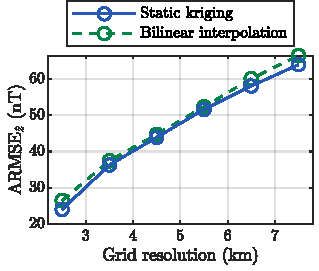
\includegraphics[width=\textwidth]{Images/ARMSE de reconstruction.pdf}

\end{column}
\begin{column}{0.47\textwidth}

\begin{block}{Static kriging against bilinear interpolation}
	\begin{itemize}
	\item Similar reconstruction errors at every resolution
	\item This suggests that the advantage of kriging in navigation lies in its reported uncertainty, not in the accuracy of the map alone
	\end{itemize}
\end{block}

\end{column}
\end{columns}

\end{frame}

\begin{frame}{Backup: kriging against bilinear, position error over time}

\centering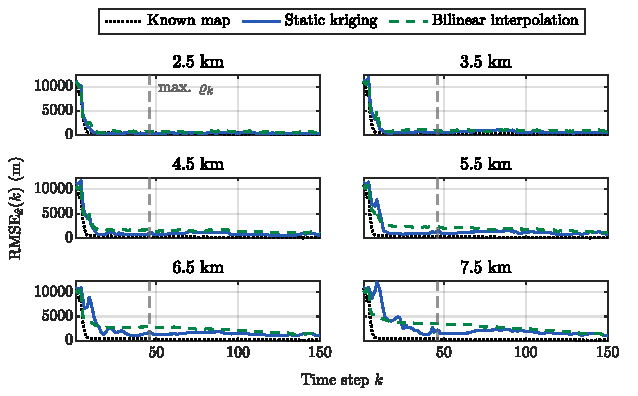
\includegraphics[width=\textwidth]{Images/RMSE par maille.pdf}

\end{frame}

\begin{frame}{Backup: kriging against bilinear, NEES over time}

\centering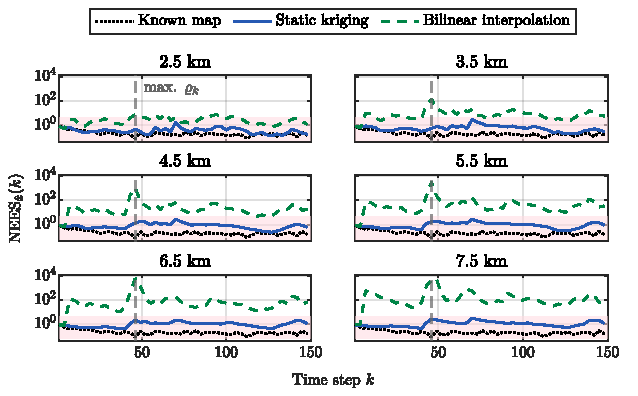
\includegraphics[width=\textwidth]{Images/NEES par maille.pdf}

\end{frame}

\begin{frame}{Backup: random subsampling, position error over time}

\centering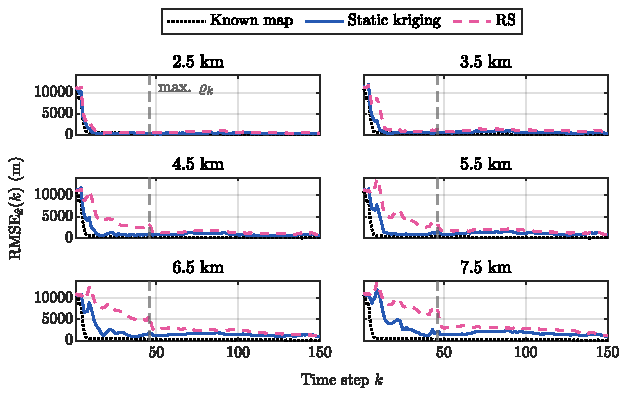
\includegraphics[width=\textwidth]{Images/RMSE eclairci par maille.pdf}

\end{frame}

\begin{frame}{Backup: random subsampling}

\begin{center}
	\scriptsize
	% Generated by figures_campagnes.m, do not edit by hand.
% Static kriging against RS.
% Analytic flop counts per run, not timings, for 5000 particles over 150 steps.
% The kriging column gathers the factorisation and the queries, which no
% method pays one without the other; the hyperparameter column is the local
% fits, and the last column, where there is one, the mean-shift of the ICAK and
% the MCAK, or
% the neighbour search of the NNAK. A method that does not pay a cost has no
% column for it.
% Where the training set is fixed, n^3/3 for the setup plus N n^2 per query.

\begin{tabular}{|c|c|c|}\hline
$\Delta_g$ & Static kriging & RS\\\hline
$2.5$ km & $29.3$ T & $7.3$ T\\
$3.5$ km & $7.39$ T & $1.84$ T\\
$4.5$ km & $2.81$ T & $704$ G\\
$5.5$ km & $1.26$ T & $314$ G\\
$6.5$ km & $608$ G & $152$ G\\
$7.5$ km & $343$ G & $85.9$ G\\
\hline
\end{tabular}

\end{center}

\begin{block}{Random subsampling, $p_{\mathrm{RS}}=0.5$}
	\begin{itemize}
	\item About $75\%$ cheaper at every resolution
	\item Systematically less accurate than static kriging
	\item Behaves as a survey of resolution $\Delta_g/\sqrt{p_{\mathrm{RS}}}$
	\end{itemize}
\end{block}

\end{frame}

\begin{frame}{Backup: AK-RPF}

\begin{block}{One iteration}
\begin{algorithmic}
	\State{$\forall i,\:x_k^{(i)}\sim p\left(\cdot\:\middle|\:x_{k-1}^{(i)}\right)$}\Comment{Particle propagation}
	\State{\textcolor{BrickRed}{$\hat{x}_{k|k-1}$ and $\hat{\mathbf{P}}_{k|k-1}$ from the weights $w_{k-1}^{(i)}$}}\Comment{\textcolor{BrickRed}{Predicted estimation}}
	\State{\textcolor{BrickRed}{Retain the survey points within $\max(r_{\mathrm{cov},k},r_{\min,k})$}}\Comment{\textcolor{BrickRed}{Adaptive subsampling}}
	\State{\textcolor{BrickRed}{$\hat{\theta}_k=\operatorname{MLE}\left(\tilde{\mathbf{x}}_{\mathrm{AK},k}^r,\tilde{\mathbf{z}}_{\mathrm{AK},k}^r,\hat{\theta}_{k-1}\right)$}}\Comment{\textcolor{BrickRed}{Hyperparameters}}
	\State{\textcolor{BrickRed}{$\forall i$, kriged likelihood $\tilde{p}\left(z_k\:\middle|\:x_k^{(i)}\right)$ on the retained points}}\Comment{\textcolor{BrickRed}{Kriging}}
	\State{$\forall i,\:w_k^{(i)}\propto w_{k-1}^{(i)}\:\tilde{p}\left(z_k\:\middle|\:x_k^{(i)}\right)$}\Comment{Weight update}
	\If{$\hat{N}_{\mathrm{eff}}<N_{\mathrm{th}}$}
	\State{Resample, then jitter the particles with the kernel}\Comment{Regularisation}
	\EndIf
\end{algorithmic}
\end{block}

\begin{block}{Settings}
	\begin{itemize}
	\item $N=5000$, $N_{\mathrm{th}}=0.5N$, $\alpha_{\mathrm{RPF}}=0.3$, $\alpha_{\mathrm{AK}}=2$, $\tilde{N}_{\min}=25$
	\item Previous hyperparameters used as initial values of the MLE
	\end{itemize}
\end{block}

\end{frame}

\begin{frame}{Backup: size of the AK window}

\begin{center}
	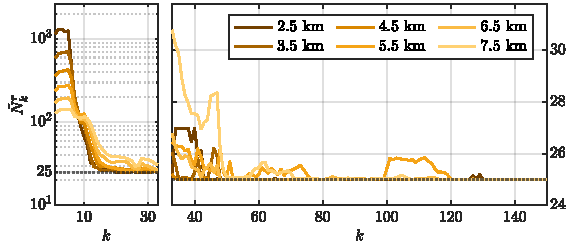
\includegraphics[width=0.9\textwidth]{Images/Echantillons retenus par maille.pdf}
\end{center}

\begin{block}{Two regimes}
	\begin{itemize}
	\item Before $k\approx25$: window set by the spread of the particles
	\item After: of the order of $\tilde{N}_{\min}=25$ points, whatever the resolution
	\end{itemize}
\end{block}

\end{frame}

\begin{frame}{Backup: costs of the window shapes}

\begin{center}
	\scriptsize
	% Generated by figures_campagnes.m, do not edit by hand.
% AK against NNAK, ICAK and MCAK.
% Analytic flop counts per run, not timings, for 5000 particles over 150 steps.
% The kriging column gathers the factorisation and the queries, which no
% method pays one without the other; the hyperparameter column is the local
% fits, and the last column, where there is one, the mean-shift of the ICAK and
% the MCAK, or
% the neighbour search of the NNAK. A method that does not pay a cost has no
% column for it.
% Two headings are abbreviated here, HP for the hyperparameter fits
% and NN for the neighbour search.
% The methods are split over two stacked tables, too many columns for
% one; both carry the same grid resolutions.
% Where the training set is fixed, n^3/3 for the setup plus N n^2 per query.

{\setlength{\tabcolsep}{3pt}%
\begin{tabular}{|c|cc|ccc|}\hline
\multirow{2}{*}{$\Delta_g$} & \multicolumn{2}{c|}{AK} & \multicolumn{3}{c|}{NNAK}\\\cline{2-3}\cline{4-6}
 & Kriging & HP & Kriging & HP & NN\\\hline
$2.5$ km & $46$ G & $564$ M & $4.3$ G & $57$ M & $47.3$ M\\
$3.5$ km & $14.4$ G & $224$ M & $2.05$ G & $36.1$ M & $43.6$ M\\
$4.5$ km & $5.75$ G & $121$ M & $1.23$ G & $25.9$ M & $40.9$ M\\
$5.5$ km & $3.09$ G & $89.8$ M & $885$ M & $21.7$ M & $38.8$ M\\
$6.5$ km & $1.93$ G & $70.1$ M & $705$ M & $19.4$ M & $36.8$ M\\
$7.5$ km & $1.54$ G & $66.7$ M & $603$ M & $18.1$ M & $35.3$ M\\
\hline
\end{tabular}
}

\par\vspace{1ex}
{\setlength{\tabcolsep}{3pt}%
\begin{tabular}{|c|ccc|ccc|}\hline
\multirow{2}{*}{$\Delta_g$} & \multicolumn{3}{c|}{ICAK} & \multicolumn{3}{c|}{MCAK}\\\cline{2-4}\cline{5-7}
 & Kriging & HP & Clustering & Kriging & HP & Clustering\\\hline
$2.5$ km & $2.26$ G & $87.3$ M & $114$ M & $24.3$ G & $340$ M & $114$ M\\
$3.5$ km & $901$ M & $83.2$ M & $158$ M & $7.61$ G & $150$ M & $158$ M\\
$4.5$ km & $616$ M & $83.3$ M & $194$ M & $3.5$ G & $97.2$ M & $195$ M\\
$5.5$ km & $547$ M & $91.4$ M & $223$ M & $2.12$ G & $76$ M & $224$ M\\
$6.5$ km & $513$ M & $107$ M & $251$ M & $1.54$ G & $66.1$ M & $253$ M\\
$7.5$ km & $499$ M & $131$ M & $270$ M & $1.25$ G & $62.4$ M & $274$ M\\
\hline
\end{tabular}
}


	\vspace{1mm}
	Flops per mission; HP: hyperparameter fits, NN: neighbour search
\end{center}

\end{frame}

\begin{frame}{Backup: number of clusters}

\begin{columns}[onlytextwidth]
\begin{column}{0.5\textwidth}

\centering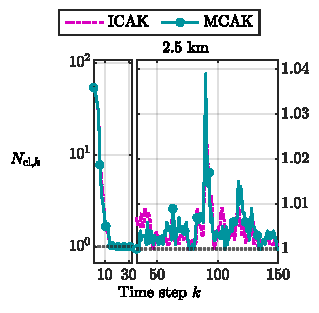
\includegraphics[width=\textwidth]{Images/Clusters fenetres par maille.pdf}

\end{column}
\begin{column}{0.47\textwidth}

\begin{block}{Mean-shift clustering}
	\begin{itemize}
	\item About $54$ clusters at $k=1$
	\item A single cluster in almost every run after about $15$ steps at $2.5$ km
	\item[$\Rightarrow$] On this scenario, ICAK and MCAK mostly reduce to AK
	\item On the EUSIPCO 2025 scenario (noises of $80$ nT, $300$ s straight line), clustering improved both accuracy and cost
	\end{itemize}
\end{block}

\end{column}
\end{columns}

\end{frame}

\begin{frame}{Backup: errors as Mahalanobis norms}

\begin{block}{Residual quantities}
	\begin{itemize}
	\item Residual kernel and residual covariance function:\\
	\hfill$\kappa_{|r}(x,x')=\kappa(x,x')-\bar{\kappa}(x,\tilde{\mathbf{x}}^r)\:\bar{\mathbf{G}}(\tilde{\mathbf{x}}^r)^{-1}\bar{\kappa}(\tilde{\mathbf{x}}^r,x'),\qquad\kappa_{d|r}(x)=\kappa_{|r}(\tilde{\mathbf{x}}^d,x)$\hfill\mbox{}
	\item Residual observation vector and its covariance:\\
	\hfill$\tilde{\mathbf{z}}_{d|r}=\tilde{\mathbf{z}}^d-\hat{z}_{\mathrm{UK}}(\tilde{\mathbf{x}}^d,\tilde{\mathbf{x}}^r,\tilde{\mathbf{z}}^r),\qquad\mathbf{S}_{d|r}=\kappa_{d|r}(\tilde{\mathbf{x}}^d)+\mathbf{I}_{\tilde{N}^d}\otimes\tilde{\mathbf{R}}$\hfill\mbox{}
	\end{itemize}
\end{block}

\begin{block}{Geometry of the errors}
	\begin{itemize}
	\item With the inner product $\langle u\mid y\rangle_{\mathbf{S}_{d|r}}\triangleq u^\top\mathbf{S}_{d|r}^{-1}y$:\\
	\hfill$\begin{gathered}
	\zeta_{\mathbf{R}}(x)=\langle\kappa_{d|r}(x)\mid\kappa_{d|r}(x)\rangle_{\mathbf{S}_{d|r}},\qquad\sigma_{\mathbf{R}}(x)=\|\kappa_{d|r}(x)\|_{\mathbf{S}_{d|r}}\\
	\zeta_{\hat{z}}(x)=\left\|\langle\kappa_{d|r}(x)\mid\tilde{\mathbf{z}}_{d|r}\rangle_{\mathbf{S}_{d|r}}\right\|_2
	\end{gathered}$\hfill\mbox{}
	\item $\|\tilde{\mathbf{z}}_{d|r}\|_{\mathbf{S}_{d|r}}^2$ follows a $\chi^2$ law with $\tilde{N}^dd_z$ degrees of freedom: the deterministic bound is looser by a factor of the order of $\sqrt{\tilde{N}^dd_z/\chi^2_{d_z}(1-\delta)}$
	\end{itemize}
\end{block}

\end{frame}

\begin{frame}{Backup: AKKF-SLAM ablation}

\begin{center}
	\scriptsize
	\renewcommand{\arraystretch}{1.15}
	\begin{tabular}{|l|c|c|}\hline
	Variant&NEES (last third)&ARMSE (km)\\\hline
	AKKF-SLAM&$11$&$1.78$\\
	Simulated observations with the sensor noise only&$15$&$1.92$\\
	Map uncertainty kept, $\alpha_{\mathrm{RKHS},Z}=0.1$&$22$&$1.96$\\
	Neither modification (FUSION 2026, moments about $\bar{x}_k$)&$57$&$2.70$\\
	Same features for the state, $\alpha_{\mathrm{RLS}}=\mathbf{R}_k/\sigma_h^2$&$2.4$&$1.71$\\\hline
	\end{tabular}
\end{center}

\begin{block}{Reading}
	\begin{itemize}
	\item Both modifications reduce the overconfidence without removing it
	\item Sharing the features between state and map brings the NEES into the band, but the field error rises to $95.0$ nT
	\end{itemize}
\end{block}

\end{frame}

\begin{frame}{Backup: SLAM results}

\begin{center}
	\scriptsize
	% Generated by figures_chapitre_5.m, do not edit by hand.
% Scenario boucle, 1000 runs, 500 particles. Position errors are averaged over
% three thirds of the mission, the NEES over the last one, and the field
% error over the evaluation points within 8 km of the trajectory.
% carte read from lot principal
% akkf_carte read from lot akkf_carte_lz1
% inertiel read from lot principal
% rbpf read from lot principal
% akkf read from lot akkf_lz1

\begin{tabular}{|l|ccc|c|c|}\hline
\multirow{2}{*}{Filter} & \multicolumn{3}{c|}{$\mathrm{ARMSE}_{\hat{x}}$ (m)} & \multirow{2}{*}{NEES} & $\mathrm{ARMSE}_{\hat{h}}$\\\cline{2-4}
 & $[\![1,100]\!]$ & $[\![101,200]\!]$ & $[\![201,300]\!]$ & & (nT)\\\hline
Known map & $183$ & $159$ & $155$ & $0.23$ & --\\\hline
Known map (AKKF) & $375$ & $102$ & $97$ & $0.06$ & --\\\hline
Inertial navigation & $1624$ & $2584$ & $3878$ & $0.04$ & $102.5$\\\hline
RBPF-SLAM & $1583$ & $1815$ & $2031$ & $9.22$ & $78.0$\\\hline
AKKF-SLAM & $1639$ & $1800$ & $1765$ & $10$ & $80.0$\\\hline
\end{tabular}

\end{center}

\begin{block}{Notes}
	\begin{itemize}
	\item NEES averaged over the last third of the mission
	\item Field error along the trajectory; for inertial navigation, the field is reconstructed as zero
	\end{itemize}
\end{block}

\end{frame}

\begin{frame}{Backup: SLAM at equal cost}

\begin{block}{AKKF-SLAM with $N=200$ particles}
	\begin{itemize}
	\item $71.2$ Gflop per run, close to the $60.9$ Gflop of RBPF-SLAM
	\item ARMSE of $2.10$ km, against $1.82$ km for RBPF-SLAM, and NEES of $24$
	\item Still $63\%$ of its runs below $2$ km against $50\%$, with $3$ MB of memory against $361$ MB
	\end{itemize}
\end{block}

\begin{block}{Why AKKF-SLAM costs more}
	\begin{itemize}
	\item The $\mathcal{O}(N^3)$ operations of the AKKF outweigh the $\mathcal{O}(N\:r_{\mathrm{KL}}^2)$ of the $N$ Kalman corrections
	\item Average computing rate: $0.48$ Gflop/s for AKKF-SLAM, $0.04$ Gflop/s for RBPF-SLAM
	\end{itemize}
\end{block}

\end{frame}

\begin{frame}{Backup: rank of the bases}

\begin{center}
	\tiny
	% Generated by figures_chapitre_5.m, do not edit by hand.
% Analytic flop counts per run, not timings, leading terms only (slam.m,
% flops_pas). Memory counts eight bytes per stored double: the N coefficient
% vectors and covariance matrices of RBPF-SLAM, the single set of AKKF-SLAM
% and three N x N matrices.

\begin{tabular}{|c|c|c|c|c|c|}\hline
Rank & $\mathrm{ARMSE}_{\hat{x}}$ (m) & NEES & $\mathrm{ARMSE}_{\hat{h}}$ (nT) & Cost (flops) & Memory (bytes)\\\hline
\multicolumn{6}{|c|}{RBPF-SLAM}\\\hline
$50$ & $7450$ & $5203$ & $328.9$ & $2.06$ G & $10.2$ M\\\hline
$100$ & $6723$ & $161$ & $168.4$ & $7.12$ G & $40.4$ M\\\hline
$200$ & $1556$ & $5.76$ & $74.7$ & $27.1$ G & $161$ M\\\hline
$300$ & $1810$ & $9.22$ & $78.0$ & $60.8$ G & $361$ M\\\hline
$400$ & $2061$ & $12$ & $78.5$ & $103$ G & $642$ M\\\hline
$500$ & $1600$ & $1.95$ & $73.4$ & $164$ G & $1$ G\\\hline
\multicolumn{6}{|c|}{AKKF-SLAM}\\\hline
$50$ & $1766$ & $13$ & $179.7$ & $638$ G & $6.02$ M\\\hline
$100$ & $1612$ & $10$ & $104.1$ & $641$ G & $6.08$ M\\\hline
$200$ & $1751$ & $11$ & $86.7$ & $650$ G & $6.32$ M\\\hline
$300$ & $1715$ & $10$ & $82.9$ & $665$ G & $6.72$ M\\\hline
$400$ & $1762$ & $11$ & $81.0$ & $686$ G & $7.28$ M\\\hline
$500$ & $1735$ & $10$ & $80.0$ & $713$ G & $8$ M\\\hline
$1000$ & $1743$ & $10$ & $77.3$ & $939$ G & $14$ M\\\hline
\end{tabular}

\end{center}

\end{frame}

\begin{frame}{Backup: references}

\begin{block}{Cited works}
	\begin{itemize}\setlength\itemsep{1mm}
	\item M. Kok, A. Solin, \emph{Scalable Magnetic Field SLAM in 3D Using Gaussian Process Maps}, FUSION 2018
	\item A. Solin, S. Särkkä, \emph{Hilbert Space Methods for Reduced-Rank Gaussian Process Regression}, Statistics and Computing, 2020
	\item T. Bailey, J. Nieto, E. Nebot, \emph{Consistency of the FastSLAM Algorithm}, ICRA 2006
	\item M. Sun, M. E. Davies, I. K. Proudler, J. R. Hopgood, \emph{Adaptive Kernel Kalman Filter}, IEEE Transactions on Signal Processing, 2023
	\item A. Rahimi, B. Recht, \emph{Random Features for Large-Scale Kernel Machines}, NeurIPS 2007
	\end{itemize}
\end{block}

\end{frame}

\end{document}
